\section{background}
XXX is compatible with OIDC, and achieves the privacy protection based on the SGX.
Here, we provide a brief introduction on OIDC and the SGX.
\subsection{OpenID Connect}
OIDC~\cite{OpenIDConnect} is an extension of OAuth 2.0 to support user authentication,
 and becomes one of the most prominent SSO authentication protocols.
Same as other SSO protocols~\cite{SAMLIdentifier}, OIDC involves three entities, i.e., {\em users}, {\em identity provider (IdP)}, and {\em relying parties (RPs)}.
Both users and RPs have to register at the IdP,    
the users register at the IdP to create credentials and identifiers (i.e. $ID_U$), 
while each RP registers at the IdP with its endpoint information to create its unique identifier (i.e., $ID_{RP}$) and the corresponding credential.
IdP is assumed to securely maintain the attributes  of users and RPs.   
Then, in the SSO authentication sessions, 
 each user is responsible to start a login request at an RP, redirect the messages between RP and IdP, and check the scope of user's attributes provided to the RP;
 IdP authenticates the user, sets the $PPID$ for the user $ID_U$ at the RP $ID_{RP}$,
 constructs the identity proof with  $PPID$, $ID_{RP}$ and the user's attributes consented by the user, and finally transmits the identity proof to the RP's registered endpoint (e.g., URL);
 each RP constructs an identity proof request with its identifier and the requested scope of  user's attributes, sends an identity proof request to the IdP through the user, and parses the received identity proof to authenticate and authorize the user.
Usually, the redirection and checking at the user are handled by a user-controlled software, called {\em user agent} (e.g., browser).

\noindent\textbf{Implicit flow of user login.}
OIDC supports three processes for the SSO authentication session, known as {\em implicit flow}, {\em authorization code flow} and {\em hybrid flow} (i.e., a mix-up of the previous two). Here, we propose the OIDC implicit flow as the example to illustrate the protocol. 

\begin{figure}[t]
  \centering
  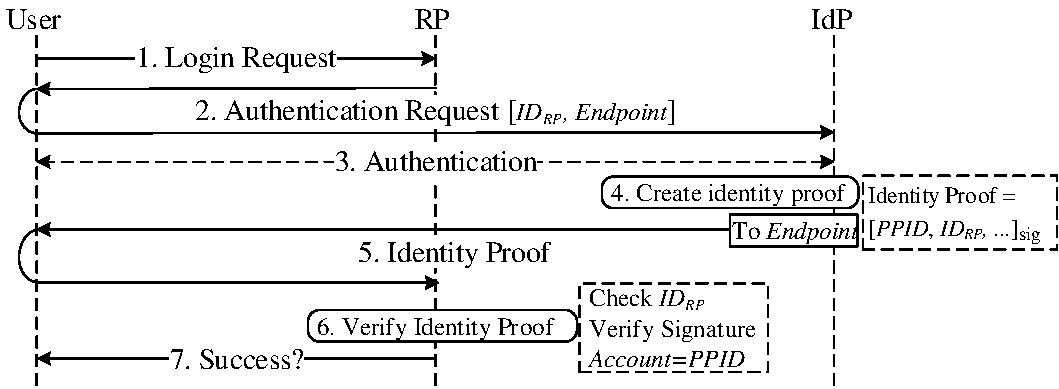
\includegraphics[width=\linewidth]{fig/OIDC1.pdf}
  \caption{The implicit protocol flow of OIDC.}
  \label{fig:OpenID}
\end{figure}

As shown in Figure~\ref{fig:OpenID}, the implicit flow of OIDC consists of 7 steps: when a user attempts to log in to an RP (Step 1), the RP constructs a request for identity proof, which is redirected by the user to the corresponding IdP (Step 2). The request contains $ID_{RP}$, RP's endpoint and a set of requested user attributes. If the user has not been authenticated yet, the IdP performs an authentication process (Step 3). If the RP's endpoint in the request matches the one registered at the IdP, it generates an identity proof (Step 4) and sends it back to the RP (Step 5). Otherwise, IdP generates a warning to notify the user about potential identity proof leakage. The RP verifies the id token (Step 6), extracts user identifier from the id token and returns the authentication result to the user (Step 7).

\subsection{Intel SGX}
Intel Software Guard Extensions (Intel SGX) is the hardware-based security  mechanism provided by Intel since the sixth generation Intel Core microprocessors, which offers memory encryption that isolates specific application code and data in memory.
It allows user-level code to allocate private regions of memory, called enclaves, which guarantees the running code are well protected from the adversary outside the enclave.
 
\noindent\textbf{Remote Attestation.} The SGX remote attestation allows a player to verify three things: the application's identity, its intactness (that it has not been tampered with), and that it is running securely within an enclave on an Intel SGX enabled platform. Moreover, with the remote attestation, the secure key exchange between the player and remote enclave application is also available even the application runs in the malicious environment.